\chapter{Обзор методов распознавания изображений} \label{chapt2}
Теория распознавания образа — раздел информатики и смежных дисциплин, развивающий основы и методы классификации и идентификации предметов, явлений, процессов, сигналов, ситуаций и т. п. объектов, которые характеризуются конечным набором некоторых свойств и признаков. Такие задачи решаются довольно часто, например, при переходе или проезде улицы по сигналам светофора. Распознавание цвета загоревшейся лампы светофора и знание правил дорожного движения позволяет принять правильное решение о том, можно или нельзя переходить улицу.

Необходимость в таком распознавании возникает в самых разных областях — от военного дела и систем безопасности до оцифровки аналоговых сигналов.

Проблема распознавания образа приобрела выдающееся значение в условиях информационных перегрузок, когда человек не справляется с линейно-последовательным пониманием поступающих к нему сообщений и в результате его голова переключается на режим одновременности восприятия и мышления, которому такое распознавание свойственно.

Неслучайно, таким образом, проблема распознавания образа оказалась в поле междисциплинарных исследований - в том числе в связи с работой по созданию искусственного интеллекта, а создание технических систем распознавания образа привлекает к себе всё большее внимание.

Распознавание образов — это отнесение исходных данных к определенному классу с помощью выделения существенных признаков, характеризующих эти данные, из общей массы несущественных данных.

Классическая постановка задачи распознавания образов: близка к постановке задачи классификации и предполагает наличие некоторого базового набора заранее известных классов (набор может расширятся), и образа (не обязательно визуального) которые надо классифицировать.

Наиболее часто в задачах распознавания визуальных образов рассматриваются монохромные изображения, что дает возможность рассматривать изображение как функцию на плоскости.

Множество же всех возможных функций f(x, y) на плоскости T — есть модель множества всех изображений X. Вводя понятие сходства между образами можно поставить задачу распознавания. Конкретный вид такой постановки сильно зависит от последующих этапов при распознавании в соответствии с тем или иным подходом.

В данной работе распознавание рассматривается в контексте задачи классификации. Можно выделить следующие классы алгоритмов для решения задачи классификации объектов

\begin{enumerate}
\item 
\end{enumerate}
%Существует множество методов распознавания изображений но в целом их можно разделить на две группы:
%\begin{enumerate}
%\item эвристические
%\item формальные
%\end{enumerate}
%
%\section{Одиночное изображение} \label{sect2_1}
%
%\begin{figure} [h] 
%  \center
%  
\includegraphics [scale=0.27] {latex}
%  \caption{TeX.} 
%  \label{img:latex}  
%\end{figure}
%
%%\newpage
%%============================================================================================================================
%\section{Длинное название параграфа, в котором мы узнаём как сделать две картинки с общим номером и названием} \label{sect2_2}
%
%А это две картинки под общим номером и названием:
%\begin{figure}[h]
%  \begin{minipage}[h]{0.49\linewidth}
%    \center{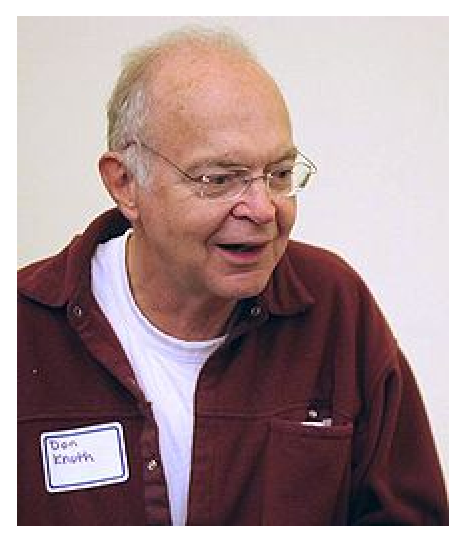
\includegraphics[width=0.5\linewidth]{knuth1} \\ а)}
%  \end{minipage}
%  \hfill
%  \begin{minipage}[h]{0.49\linewidth}
%    \center{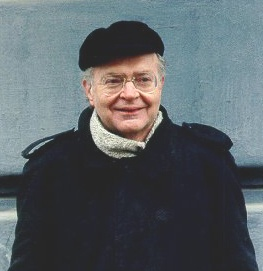
\includegraphics[width=0.5\linewidth]{knuth2} \\ б)}
%  \end{minipage}
%  \caption{Очень длинная подпись к изображению, на котором представлены две фотографии Дональда Кнута}
%  \label{img:knuth}  
%\end{figure}
%
%%\newpage
%%============================================================================================================================
%\section{Пример вёрстки списоков} \label{sect2_3}
%
%\noindent Нумерованный список:
%\begin{enumerate}
%  \item Первый пункт.
%  \item Второй пункт.
%  \item Третий пункт.
%\end{enumerate}
%
%\noindent Маркированный список:
%\begin{itemize}
%  \item Первый пункт.
%  \item Второй пункт.
%  \item Третий пункт.
%\end{itemize}
%
%\noindent Вложенные списки:
%\begin{itemize}
%  \item Имеется маркированный список.
%  \begin{enumerate}
%    \item В нём лежит нумерованный список,
%    \item в котором
%    \begin{itemize}
%      \item лежит ещё один маркированный список.
%    \end{itemize}    
%  \end{enumerate}
%\end{itemize}
%
%
%\clearpage